\section{Read In}
\label{sec:lit}

A chosen topic makes a debt: the literature.
Our rules for the literature review are few.
Figure~\ref{fig:prompt} shows the full prompt.
The first three lines are configuration that machines read.
The rules drive the pipeline.

\begin{figure}[t]
\fbox{\parbox{\dimexpr\linewidth-2\fboxsep-2\fboxrule}{\small
{\ttfamily goal:~~human factors of AI assistants\\ \hspace*{4.2em}for
[software engineering]\\ years:~2021-2026\\ seed:~~the team's three
in-query papers}\\[0.4em] Rules: (1)~let the speed of the field set
``recent'': ten years usually, two to three years for LLM-speed
fields; (2)~the term in brackets is a venue filter: the first search
looks only in the venues of that field, from a venue list that a human
can review;\footnote{Sources for the list: se-deadlines.github.io, the
venue index of Google Scholar for ``software engineering,'' OpenAlex
sources with ``software'' in their names, and the venues of the team's
own recent papers.
CORE does not list journals now.}
(3)~sort the hits by citations, and read above the knee of that curve
(the point farthest from the first-to-last chord); (4)~seeds go into
the reading set without a citation test; (5)~the snowball has no venue
filter: it walks backward from the reading set to the classics, and
forward from the seeds to the newest work; (6)~the download rate is a
finding: report it, and never drop missing papers without a word.
Then code each abstract; look for subsets and their overlaps; and list
the papers of the team that already sit inside the set.}}
\caption{The prompt that runs the literature review (from the
search rules of the rite engine, github.com/timm/rite).}
\label{fig:prompt}
\end{figure}

\begin{figure}[t]
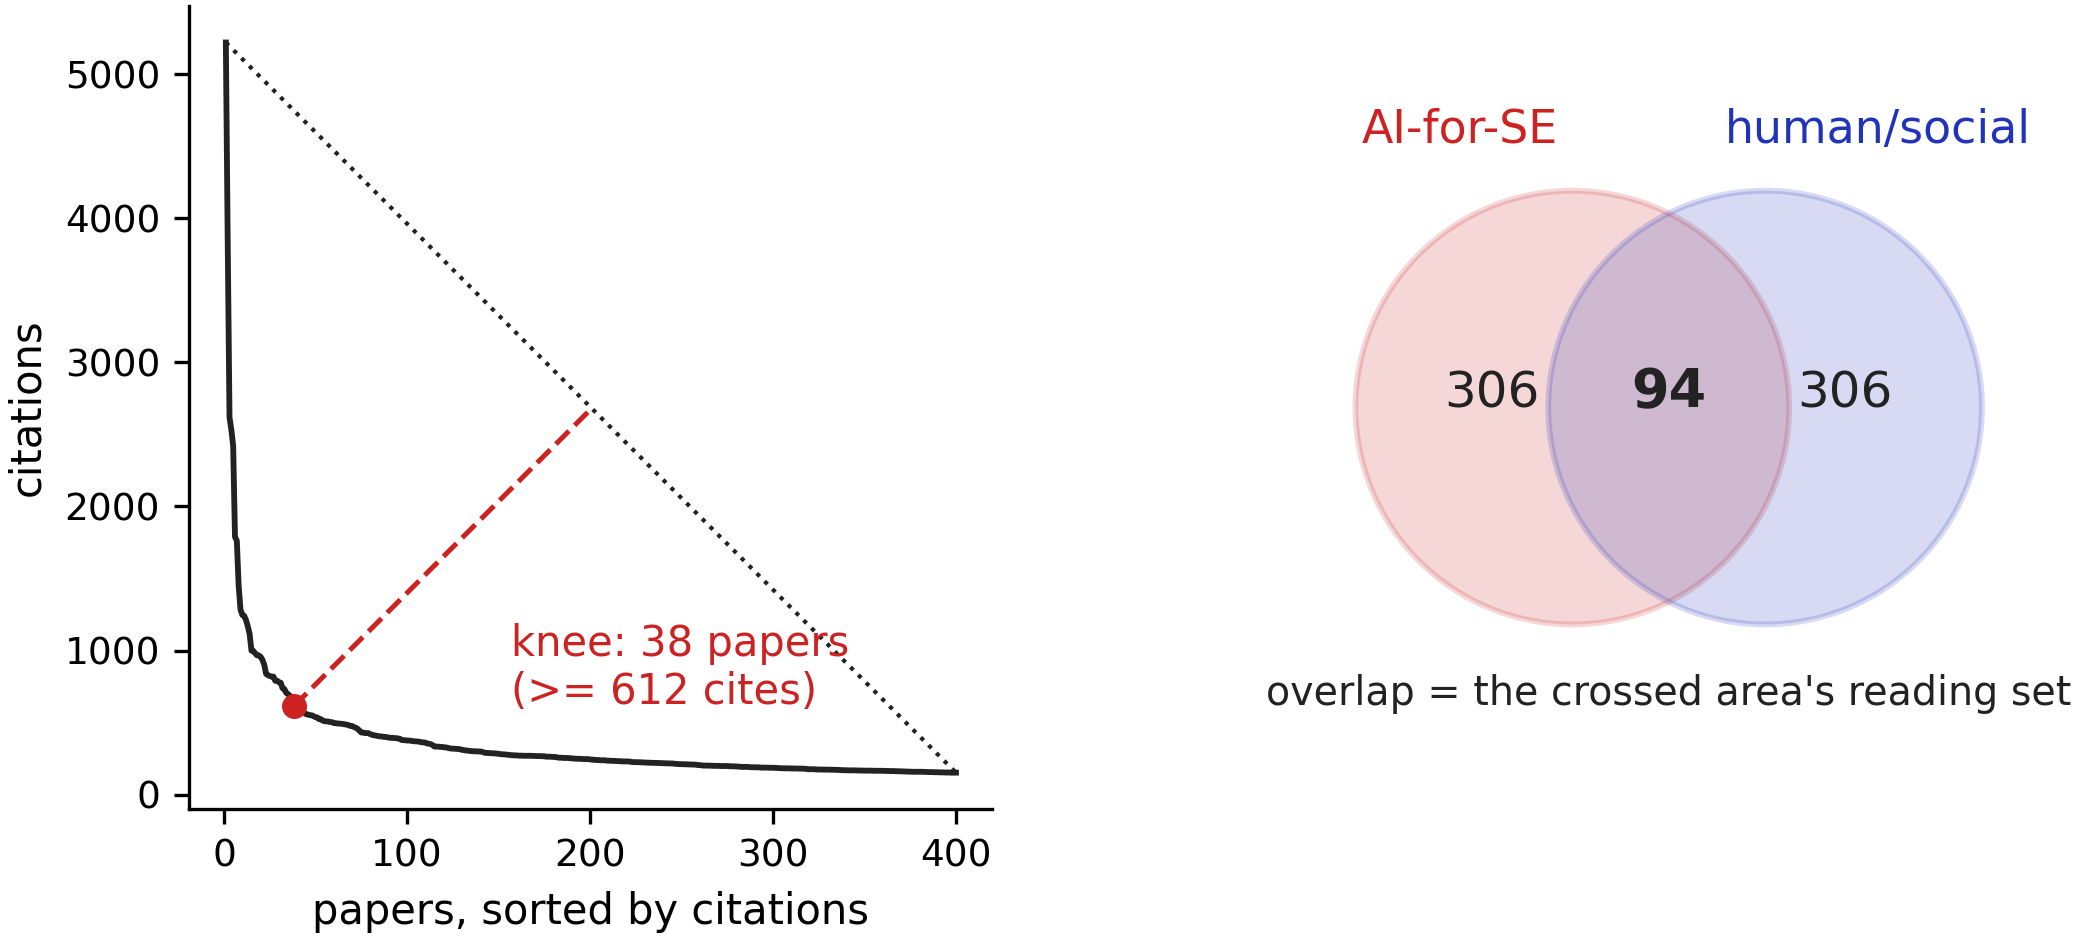
\includegraphics[width=\linewidth]{fig/lit}
\caption{Left: the sorted-cites curve of the goal query, searched
only in SE venues (\litSE{} papers, OpenAlex, 2021--2026).
The dotted line goes from the most-cited to the least-cited paper.
The dashed drop marks the point farthest from that line: the knee,
\litKnee{} papers at \litKneeCites{} citations or more.
Right: the two wings as different queries, with the same venues, and
their \litBoth-paper overlap.
To make this figure again, use {\em make lit}.}
\label{fig:lit}
\end{figure}

Figure~\ref{fig:lit} shows the rules on the area that \S\ref{sec:map}
selected.
The venue rule earned its place two times.
A first draft skipped the rule.
The reading set then filled with general AI blockbusters, and their
venues were far from software engineering.
A second draft filtered the venues after a citation-sorted fetch.
That also failed.
Of the top 1{,}000 hits, only nine sat in SE venues, because papers
with very many citations push out the field before the filter runs.
Thus, the venue list goes into the query itself.
The human hours go only to papers that our field knows.

\begin{figure}[t]
\centering
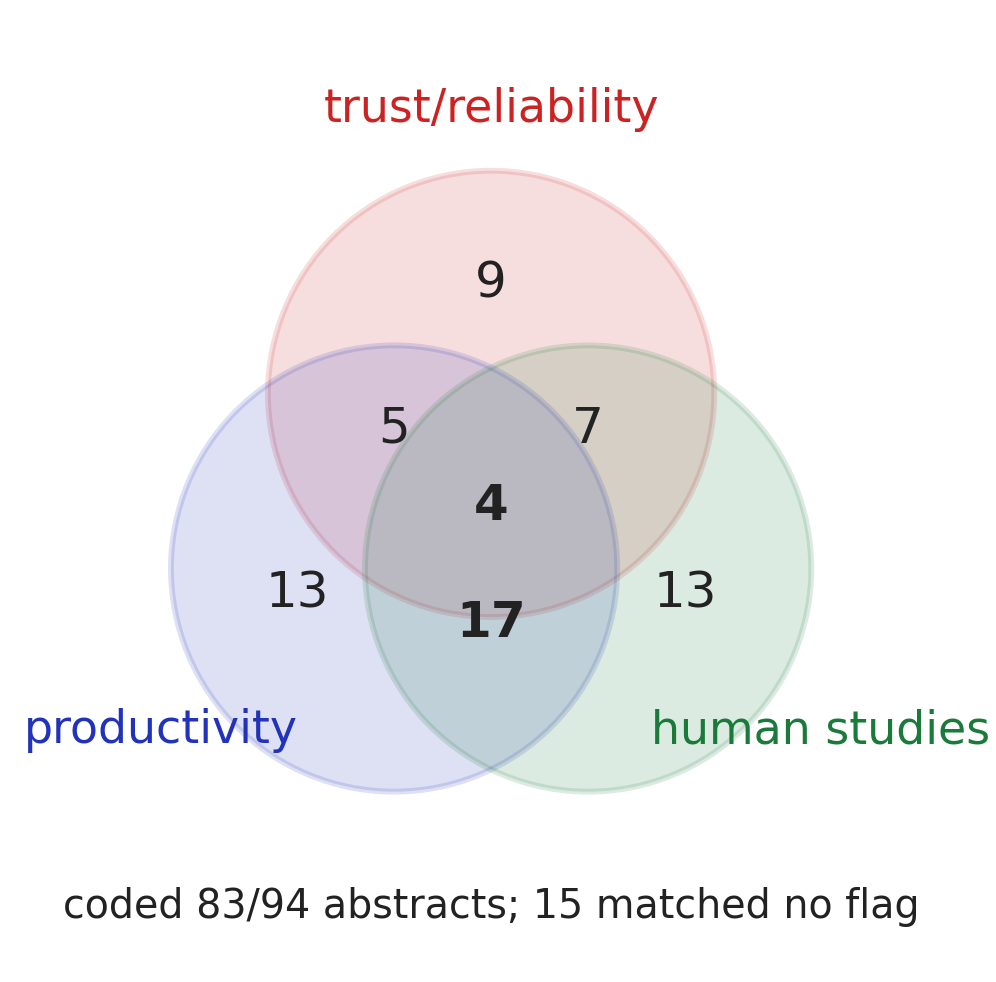
\includegraphics[width=0.62\linewidth]{fig/lit2}
\caption{The reading set (the \litKnee{} papers above the knee of
Figure~\ref{fig:lit}, plus three seeds), coded against three topic
flags.
To make this figure again, use {\em make lit}.}
\label{fig:lit2}
\end{figure}

The reading set is the papers above the knee, plus the seeds.
Rule~(4) admits the seeds without a citation test.
Here, the seeds are the three papers of the team inside the query (the
rows with ``s'' in Table~\ref{tab:read}).
The set has \litRead{} papers, and \litAbs{} of them have abstracts.
Figure~\ref{fig:lit2} codes those abstracts with three topic flags
(trust, productivity, human method).
\litTPH{} papers sit in all three circles, and \litNone{} papers match
no flag.
Table~\ref{tab:read} lists the set and its flags.

\begin{table*}[t]
\caption{The reading set: title (first author), venue, year,
citations, and the three topic flags of Figure~\ref{fig:lit2}.
The rows with ``s'' are seeds: the papers of the team inside the
query, admitted without a citation test. {\em litfig.py} makes this
table from OpenAlex, with the venues as recorded there.}
\label{tab:read}
\scriptsize \setlength{\tabcolsep}{3pt}
\centering
% generated by litfig.py; do not hand-edit
\begin{tabular}{@{}rp{0.58\linewidth}p{0.17\linewidth}rr@{}}
\toprule
\# & paper & venue & year & cites\\
\midrule
1 & Machine Learning: Algorithms, Real-World Application... (Sarker) & SN Computer Science & 2021 & 5221\\
2 & Opinion Paper: “So what if ChatGPT wrote it?” Multid... (Dwivedi) & International Journal  & 2023 & 3869\\
3 & Metaverse beyond the hype: Multidisciplinary perspec... (Dwivedi) & International Journal  & 2022 & 2619\\
4 & Machine learning and deep learning (Janiesch) & Electronic Markets & 2021 & 2534\\
5 & GPT-4 Technical Report (OpenAI) & arXiv (Cornell Univers & 2023 & 2421\\
6 & A Metaverse: Taxonomy, Components, Applications, and... (Park) & IEEE Access & 2022 & 1789\\
7 & Natural language processing: state of the art, curre... (Khurana) & Multimedia Tools and A & 2022 & 1762\\
8 & ARTIFICIAL INTELLIGENCE FOR THE REAL WORLD (?) & International Research & 2023 & 1450\\
9 & A survey on large language model based autonomous ag... (Wang) & Frontiers of Computer  & 2024 & 1284\\
10 & Flamingo: a Visual Language Model for Few-Shot Learn... (Jean-Baptiste) & arXiv (Cornell Univers & 2022 & 1247\\
11 & Generative AI (Feuerriegel) & Business \& Informatio & 2023 & 1241\\
12 & A SWOT analysis of ChatGPT: Implications for educati... (Farrokhnia) & Innovations in Educati & 2023 & 1212\\
13 & A Review of Artificial Intelligence (AI) in Educatio... (Zhai) & Complexity & 2021 & 1168\\
14 & AI-Based Modeling: Techniques, Applications and Rese... (Sarker) & SN Computer Science & 2022 & 1114\\
15 & Hydrogen production, storage, utilisation and enviro... (Osman) & Environmental Chemistr & 2021 & 999\\
16 & Deep learning modelling techniques: current progress... (Ahmed) & Artificial Intelligenc & 2023 & 997\\
17 & The future landscape of large language models in med... (Clusmann) & Communications Medicin & 2023 & 981\\
18 & Unmanned aerial vehicles (UAVs): practical aspects, ... (Mohsan) & Intelligent Service Ro & 2023 & 967\\
19 & A Survey on the Explainability of Supervised Machine... (Burkart) & Journal of Artificial  & 2021 & 966\\
20 & New Era of Artificial Intelligence in Education: Tow... (Kamalov) & Sustainability & 2023 & 956\\
21 & Artificial intelligence and smart vision for buildin... (Baduge) & Automation in Construc & 2022 & 935\\
22 & Using machine learning approaches for multi-omics da... (Reel) & Biotechnology Advances & 2021 & 900\\
23 & A Review of the Role of Artificial Intelligence in H... (Kuwaiti) & Journal of Personalize & 2023 & 838\\
24 & Unlocking the value of artificial intelligence in hu... (Chowdhury) & Human Resource Managem & 2022 & 829\\
25 & A survey on deep learning tools dealing with data sc... (Alzubaidi) & Journal Of Big Data & 2023 & 823\\
26 & Smart wearable devices in cardiovascular care: where... (Bayoumy) & Nature Reviews Cardiol & 2021 & 819\\
27 & Adaptive Learning Using Artificial Intelligence in e... (Gligorea) & Education Sciences & 2023 & 819\\
28 & <scp>ChatGPT</scp> and a new academic reality: <scp>... (Lund) & Journal of the Associa & 2023 & 790\\
29 & Human resource management in the age of generative a... (Budhwar) & Human Resource Managem & 2023 & 790\\
30 & Challenges and Opportunities of Generative AI for Hi... (Michel‐Villarreal) & Education Sciences & 2023 & 780\\
31 & Survey on 6G Frontiers: Trends, Applications, Requir... (Alwis) & IEEE Open Journal of t & 2021 & 776\\
32 & A Review on Large Language Models: Architectures, Ap... (Raiaan) & IEEE Access & 2024 & 738\\
33 & AI Tools in Society: Impacts on Cognitive Offloading... (Gerlich) & Societies & 2025 & 732\\
34 & Academic Integrity considerations of AI Large Langua... (Perkins) & Journal of University  & 2023 & 706\\
35 & ChatGPT and Open-AI Models: A Preliminary Review (Roumeliotis) & Future Internet & 2023 & 697\\
36 & Retrieval-Augmented Generation for Large Language Mo... (Gao) & arXiv (Cornell Univers & 2023 & 686\\
37 & The impact of big data analytics and artificial inte... (Benzidia) & Technological Forecast & 2021 & 675\\
38 & Teachers’ AI digital competencies and twenty-first c... (Ng) & Educational Technology & 2023 & 612\\
\bottomrule
\end{tabular}

\end{table*}

Then the snowball runs from that set.
The snowball has no venue filter, because good ancestors and good
critics live in all venues.
The backward walk found \litRefs{} different references.
Of these, \litClassics{} have two or more citers inside the reading
set, and those are the candidate classics.
The forward walk found \litCiting{} works that already cite the
reading set.
\note{timm}{the three flags are paper0-local; a full run would fork
its own workdir and flags.py, per the engine rules}

The process itself gave findings.
Full texts are rare.
In the companion run of this workdir, only 22 of 54 wanted PDFs (41\%)
downloaded.
Abstracts come more easily (here, \litAbs{} of \litRead).
Google Scholar does not speak to scripts.
OpenAlex, Semantic Scholar, and arXiv answer machine queries.
Thus, the pipeline stands only on the willing.
An earlier full-text pass showed that abstract-only coding missed
about half of the flags.
Thus, we code the full text above the knee.
Last, the own-papers rule paid.
Three papers of this team already sit in the results (Di Nucci on
accessibility, Schmid on MLOps, Esposito on AI agents).
The territory is adjacent to us, but we do not occupy it yet.

\begin{pause}{the search}
Ask: are the goal line and the two wing queries the correct words?
Is 2021 the correct floor for ``recent''?
Is the venue list (see the box) the SE that you know?
Are the three coding flags your vocabulary, and is a knee that keeps
\litKnee{} of \litSE{} papers too greedy?\\[0.2em] To change the
outcome: edit the query strings, {\ttfamily VENUES}, and {\ttfamily
FLAGS} in {\ttfamily litfig.py}; remove the cache in {\ttfamily tmp/};
then run again.
The two figures, the table, and each number in this section change
with them.
\end{pause}
